\section{Forudsigelse af indlæggelsesvarigheden}
Ved ortopædkirurgiske operationer er der flere parametre, der kan have indflydelse på indlæggelsesvarigheden. Dette kan eksempelvis være demografiske parametre såsom alder samt køn og kliniske parametre som blodprøver, blodtab og operationstype. Da der kan opstå komplikationer under en operationen, som kan have indflydelse på indlæggelsesvarigheden opdeles parametrene i præ- og postoperativt.


\subsection{Præoperativt}
På ortopædkirurgisk afdeling estimeres indlæggelsesvarigheden ikke på nuværende tidspunkt, dog vurderes indlæggelsesforløbet ud fra personalets erfaringer. Ud fra informationspjecer fra ortopædkirurgisk afdeling på Aalborg Universitetshospital samt studier der har påvist at demografiske, livsstilfaktorer samt kliniske faktorer, kan medfører komplikationer under en operation. Disse kan angiveligt medfører forlænget indlæggelsesvarighed. 


\subsubsection{Demografiske}
Livsstilsfaktorer tyder på, at have betydning for komplikationer under en operation. En faktor som lavt funktionsniveau og muskeltab, som ofte er aldersbetinget, kan medfører komplikationer og derved længere indlæggelsesvarighed. Hvorimod patienter med højt funktionsniveau ofte har kortere indlæggelsesvarighed.\cite{Kehlet2001, Janssen2002} Af \figref{alderogindlaeggelse} fremgår sammenhængen mellem patienters alder og indlæggelsesvarighed. 


\begin{figure}[H]
	%\flushleft 
	\centering
	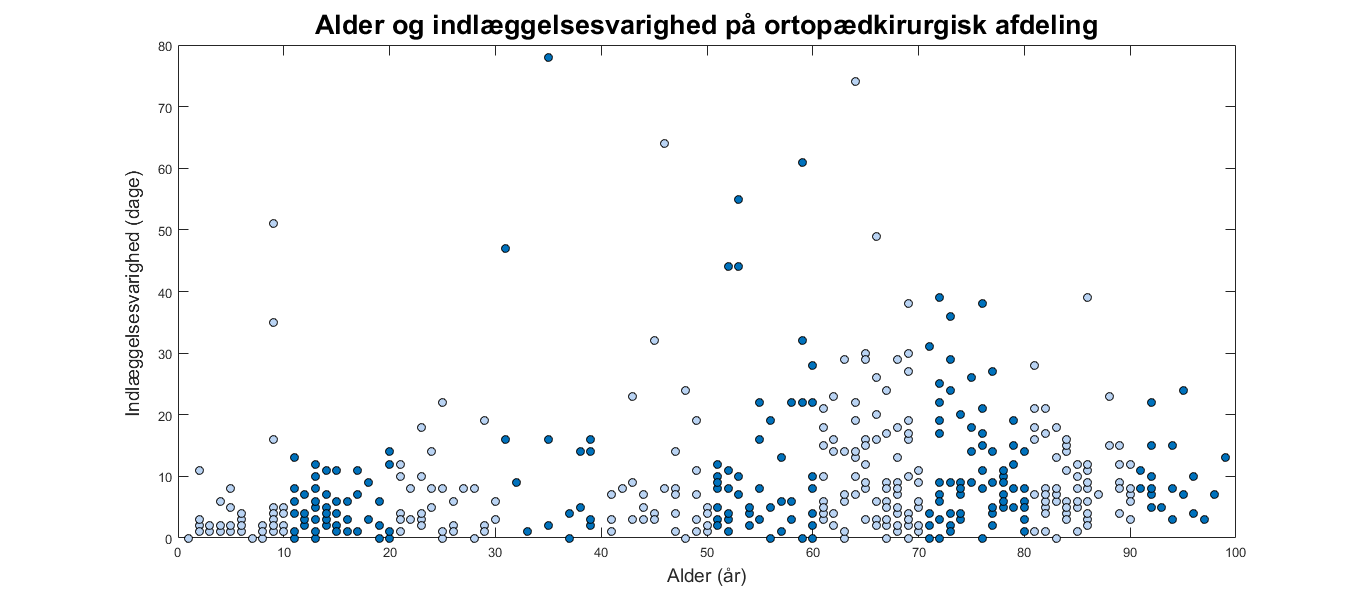
\includegraphics[scale=0.5]{figures/alderogindlaeg}
	%\flushleft
	\caption{\textit{Alder og indlæggelsesvarighed for patienter på ortopædkirurgisk afdeling. Dette er over en periode på 3 måneder fra den 1. august til den 31. oktober år 2014.}}
	\label{alderogindlaeggelse}
\end{figure}


\noindent
På \figref{alderogindlaeggelse} ses det, at der er en bred aldersfordeling på ortopædkirurgisk afdeling. Derudover fremgår det, at indlæggelsesvarigheden for ældre patienter er mere varierende end yngre patienter, hvoraf denne variation stiger med alderen. Det fremgår ligeledes, at de ældre patienter indlægges i længere tid end yngre patienter. Patienter under $30$ år er i gennemsnit indlagt 5 dage, hvor patienter over $30$ år i gennemsnit er indlagt 10,9 dage. Det er uvist om, dette skyldes lavt funktionsniveau eller om der er andre faktorer der spiller ind. Eksempelvis kan der være forskel på, hvilken operation der foretages på ældre fremfor yngre patienter, hvilket kan medvirke til den øgede indlæggelsesvarighed.

For at teste for om der er signifikant sammenhæng mellem alder og indlæggelsesvarighed, foretages en to sample t-test. Resultaterne af denne test fremgår af \tabref{alderogindlaegtab}.

\begin{table}[H]
\centering
\begin{tabular}{|c|c|c|c|}
\hline
\multicolumn{1}{|l|}{\textbf{Alder (år)}} & \multicolumn{1}{l|}{\textbf{Sub-sample}} & \multicolumn{1}{l|}{\textbf{Indlæggelsesgennemsnit}} & \multicolumn{1}{l|}{\textbf{P-værdi}} \\ \hline
0-10                                      & 46                                       & 4,67                                                 & 0,0021*                               \\ \hline
11-20                                     & 55                                       & 4,56                                                 & 4,9727                                \\ \hline
21-30                                     & 36                                       & 5,89                                                 & 0,0280*                               \\ \hline
31-40                                     & 17                                       & 13,71                                                & 0,0483*                               \\ \hline
41-50                                     & 34                                       & 9,00                                                 & 0,4470                                \\ \hline
51-60                                     & 52                                       & 11,65                                                & 0,0637                                \\ \hline
61-70                                     & 91                                       & 12,04                                                & 0,0105*                               \\ \hline
71-80                                     & 73                                       & 10,95                                                & 0,0948                                \\ \hline
81-90                                     & 62                                       & 9,47                                                 & 0,4362                            \\ \hline
91-100                                    & 20                                       & 9,50                                                 & 0,4574                                \\ \hline
\end{tabular}
\caption{Statistik over sammenhæng mellem indlæggelsesvarigheden og alder. P-værdier under et signifikantsniveau på 5\% er angivet med *.}
\label{alderogindlaegtab}
\end{table}

\noindent
Af \ref{alderogindlaegtab} ses p-værdier for sammenhængen mellem indlæggelsesvarigheden og alder. Det fremgår, at aldergrupperne 0 til 10 år, 21 til 30 år, 31 til 40 år samt 61 til 70 år har en statistisk indflydelse på indlæggelsesvarigheden. Patienter der er mellem 0 år og 10 år samt 21 år og 30 år ligger i gennemsnit kortere tid end den gennemsnitlige patient. Derudover er patienter mellem 31 år og 40 år samt 61 og 70 år er indlagt længere tid end gennemsnittet. Det tyder derfor på, at der er en sammenhæng mellem alder og indlæggelsesvarigheden inden for disse aldersgrupper.


\subsubsection{Livsstilfaktorer}
Udover deomgrafiske faktorer kan livsstilsfaktorer, som vægt, have en indflydelse på operationer foretaget på ortopædkirurgisk afdeling, da overvægt giver større risiko for blodpropper\cite{Ermonds2004}. Ved overvægt anbefales det derved at tabe sig før en eventuel operation. Foruden mindsket risiko ved opstående komplikationer, kan smerter ligeledes reduceres ved vægttab.\cite{Nordjylland2014} På \figref{BMIogindlaeggelse} fremgår sammenhængen mellem body mass index (BMI) og indlæggelsesvarigheden.

\begin{figure}[H]
	%\flushleft 
	\centering
	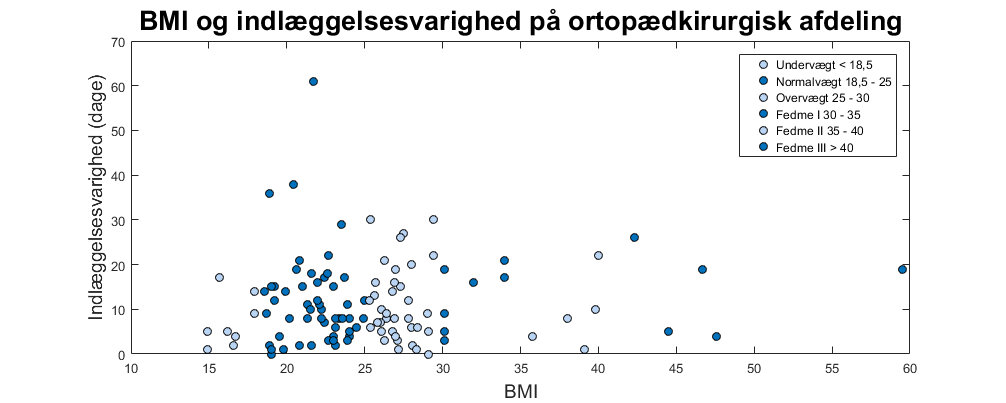
\includegraphics[scale=0.55]{figures/BMIogindlaeg}
	%\flushleft
	\caption{\textit{BMI og indlæggelsesvarighed for patienter på ortopædkirurgisk afdeling. BMI er opdelt i 6 kategorier: Undervægtig, normalvægtig, overvægt, fedme I, fedme II og fedme III. Dette er over en periode på 3 måneder fra den 1. august til den 31. oktober år 2014.}}
	\label{BMIogindlaeggelse}
\end{figure}

\noindent
Af \figref{BMIogindlaeggelse} fremgår det, at størstedelen af patienterne på ortopædkirurgisk afdeling befinder sig inden for vægtklassen normal og overvægtig. I disse klasser er indlæggelsesvarigheden mere varierende end de resterende klasser, hvor patienterne her er indlagt fra 0 til 61 dage. Dette kan skyldes at samplestørrelsen i de resterende klasser er mindre, hvorfor der ved en større sample kan være samme variation. 
Den gennemsnitlige indlæggelses tid for normalvægt og overvægt er 11,3 dage, mens den for fedmeklasse I, II og III i gennemsnit er 11,7 dage. Det tyder derfor på, at et højere BMI ikke har en betydning for en længere indlæggelsesvarighed. 


For at teste om BMI har indflydelse på indlæggelsesvarigheden udføres der en to sample t-test. Resultaterne heraf fremgår af \tabref{BMIogindlaegtab}.

\begin{table}[H]
\centering
\begin{tabular}{|c|c|c|c|}
\hline
\textbf{BMI}         & \textbf{Sub-sample} & \textbf{Indlæggelsesgennemsnit} & \textbf{P-værdi} \\ \hline
Undervægt \textless18.5  & 19                  & 11,37                           & 0,4953           \\ \hline
Normalvægt 18.5 - 25     & 77                  & 11,48                           & 0,4581           \\ \hline
Overvægt 25-30           & 47                  & 11,13                           & 0,4432           \\ \hline
Fedme I 30-35            & 15                  & 12,40                           & 0,3357           \\ \hline
Fedme II 35-40           & 6                   & 8,00                            & 0,1899           \\ \hline
Fedme III \textgreater40 & 5                   & 14,60                           & 0,2180           \\ \hline
\end{tabular}
\caption{Statistik over sammenhæng mellem indlæggelsesvarigheden og BMI. P-værdier under et signifikantsniveau på 5\% er angivet med *.}
\label{BMIindlaegtab}
\end{table}

\noindent
Det fremgår af \ref{BMIindlaegtab}, at der ikke er nogen statistisk sammenhæng mellem indlæggelsesvarigheden og BMI. Det vil sige, at dette kan være en parameter der ikke har nogen indflydelse på, hvor længe patienterne er indlagt.

Andre livsstilsfaktorer såsom rygning og alkohol kan have betydning for komplikationer under operationer. Rygning kan være medvirkende til at knogler og sår heler langsommere. Ved operationer, hvor der skal transplanteres knoglevæv, f.eks. rygoperationer, afhænger resultat af operation af, at knoglevævet heler rigtigt. Det anbefales at stoppe med at ryge 6 måneder før en operation, hvorfor en ikke ryger defineres som en person der har været røgfri i 6 måneder før den planlagte operationen.\cite{Nordjylland2014} Fordelingen af aktive rygere, tidligere rygere og ikke rygerere samt sammenhængen mellem, hvilken betydning dette har for indlæggelsesvarigheden fremgår af \figref{rygningogindlaeggelse}.


\begin{figure}[H]
	%\flushleft 
	\centering
	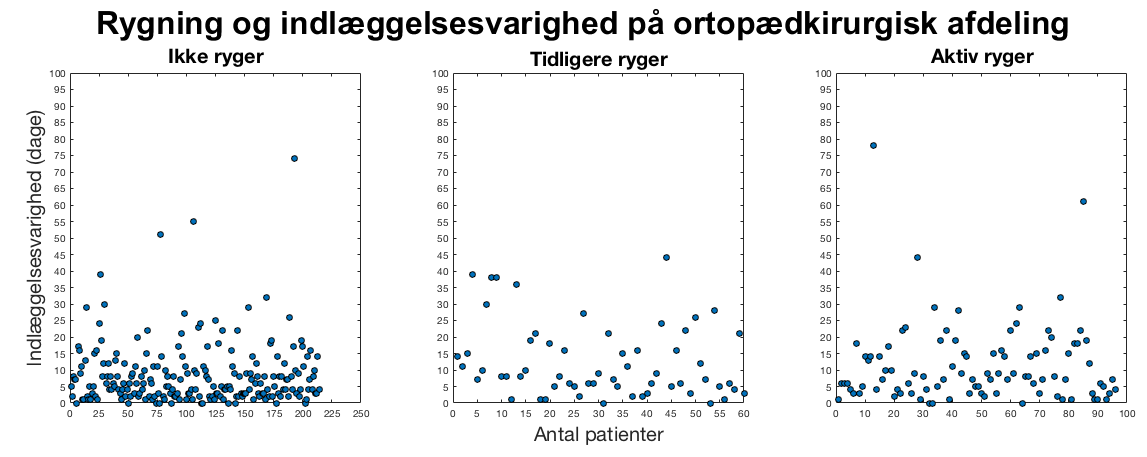
\includegraphics[scale=0.5]{figures/rygerogindlaeg}
	%\flushleft
	\caption{\textit{Rygning og indlæggelsesvarighed for patienter på ortopædkirurgisk afdeling. Rygning er opdelt efter ikke ryger, eks ryger og aktiv ryger. Eks ryger defineres som røgfri i et halvt år. Dette er over en 3 måneders periode fra den 1. august til den 31. oktober år 2014.}}
	\label{rygningogindlaeggelse}
\end{figure}


\noindent
Det ses af \figref{rygningogindlaeggelse}, at størstedelen af patienterne som indlægges på ortopædkirurgisk afdeling ikke ryger. Derudover fremgår det, at variationen i indlæggelsesvarigheden er større for eks rygere og rygere end for aktive rygere. Den gennemsnitlige indlæggelsesvarighed er for ikke rygere 8,4 dage, hvor den for eks rygere og aktive rygere er, henholdsvis 12,8 og 11 dage. Det tyder derfor på, at rygning har en betydning for indlæggelsesvarigheden. 

Dertil undersøges der om der er en statistisk sammenhæng mellem indlæggelsesvarigheden og rygning, hvortil der udføres en to sample t-test, som fremgår af \ref{rygerindlaegtab}.

\begin{table}[H]
\centering
\begin{tabular}{|c|c|c|c|}
\hline
\textbf{Ryger} & \textbf{Sub-sample} & \textbf{Indlæggelsesgennemsnit} & \textbf{P-værdi} \\ \hline
Ikke ryger        & 296                 & 8,3649                          & 0,0324*          \\ \hline
Eks ryger         & 84                  & 12,8095                         & 0,0072*          \\ \hline
Ryger             & 123                 & 11,0325                         & 0,1186           \\ \hline
\end{tabular}
\caption{Statistik over sammenhæng mellem indlæggelsesvarigheden og rygning. P-værdier under et signifikantsniveau på 5\% er angivet med *.}
\label{rygerindlaegtab}
\end{table}

\noindent
På \ref{rygerindlaegtab} ses det, at aktive rygninger ikke har en indflydelse på indlæggelsesvarigheden, mens eks rygere og ikke rygere har en statistisk indflydelse på indlæggelsesvarigheden. Eks rygere er i gennemsnit indlagt længere tid end gennemsnittet, mens det ikke-rygere modsat er indlagt kortere tid end gennemsnittet. Det kan derfor tyde på, at indlæggelsesvarighden for patienter forkortes, hvis patienten ikke ryger. 

Som tidligere nævnt kan alkohol ligeledes medføre øget risiko for komplikationer under operationer. Herunder kan der opstå øget blødning under operationer samt infektioner i såret.\cite{Nordjylland2014} Sammenhængen mellem alkohol og indlæggelsesvarigheden er illustreret på  \figref{alkohologindlaeggelse}. 


\begin{figure}[H]
	%\flushleft 
	\centering
	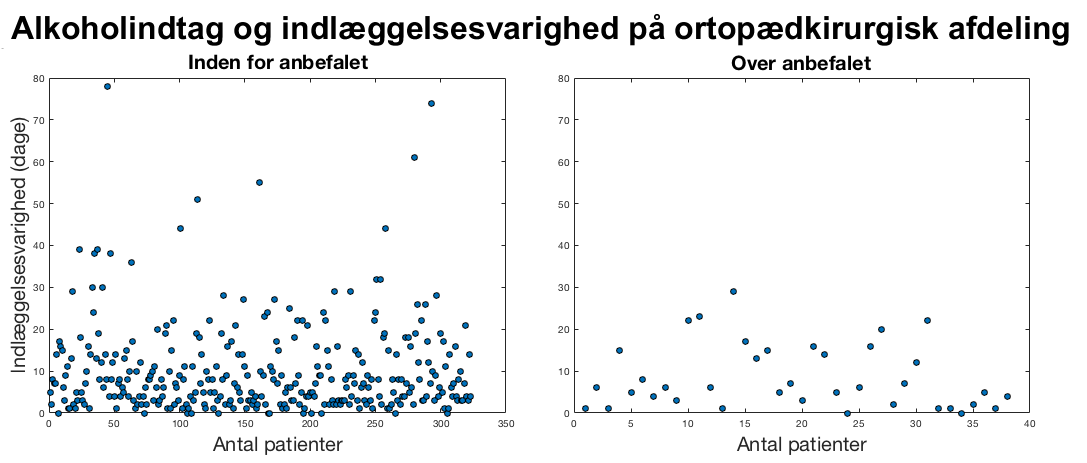
\includegraphics[scale=0.4]{figures/alkohologindlaeg}
	%\flushleft
	\caption{\textit{Alkohol og indlæggelsesvarighed for patienter på ortopædkirurgisk afdeling. Alkohol er opdelt i inden for anbefalet og over anbefalet. Dette er over en periode på 3 måneder fra den 1. august til den 31. oktober år 2014. }}
	\label{alkohologindlaeggelse}
\end{figure}

\noindent
Det fremgår af \figref{alkohologindlaeggelse}, at størstedelen af patienter på ortopædkirurgisk afdeling befinder sig inden for anbefalingen af alkoholindtag. Den gennemsnitlige indlæggelsesvarighed for patienter, der holder sig inden for det anbefalede er 10 dage, mens den for patienter der drikker over anbefalet er indlagt 8,4 dage. Det tyder derfor på, at patienter der drikker inden for anbefalet er indlagt i længere tid end patienter der over anbefalet. 
For at kunne bekræfte denne sammenhæng udføres en to sample t-test. Resultatet af denne test fremgår af \ref{alkoholindlaegtab}


\begin{table}[H]
\centering
\begin{tabular}{|c|c|c|c|}
\hline
\textbf{Alkohol} & \textbf{Sub-sample} & \textbf{Indlæggelsesgennemsnit} & \textbf{P-værdi} \\ \hline
Under anbefalet   & 443                 & 10,01                           & 0,4154           \\ \hline
Over anbefalet    & 47                  & 8,45                            & 0,1882           \\ \hline
\end{tabular}
\caption{Statistik over sammenhæng mellem indlæggelsesvarigheden og alkohol. P-værdier under et signifikantsniveau på 5\% er angivet med *.}
\label{alkoholindlaegtab}
\end{table}

\noindent
Det fremgår af \ref{alkoholindlaegtab}, at der ingen statistisk sammenhæng er mellem alkohol og indlæggelsesvarigheden. Dette kan skyldes, at det er en subjektiv vurdering, hvorfor egen holdning kan have indflydelse på patientens svar. 

Det tyder på, at livsstilsfaktorer som komorbiditeter har betydning for indlæggelsesvarigheden. Patienter med komorbiditeter f.eks. dårligt blodomløb og diabetes ofte kræver særlig behandling, hvilket medfører længere indlæggelse. Diabetes har bl.a. betydning ift. sårheling \ref{bilagA}. Af figur \figref{diabetesogindlaeggelse} fremgår sammenhængen mellem diabetes og indlæggelsesvarigheden. 

\begin{figure}[H]
	%\flushleft 
	\centering
	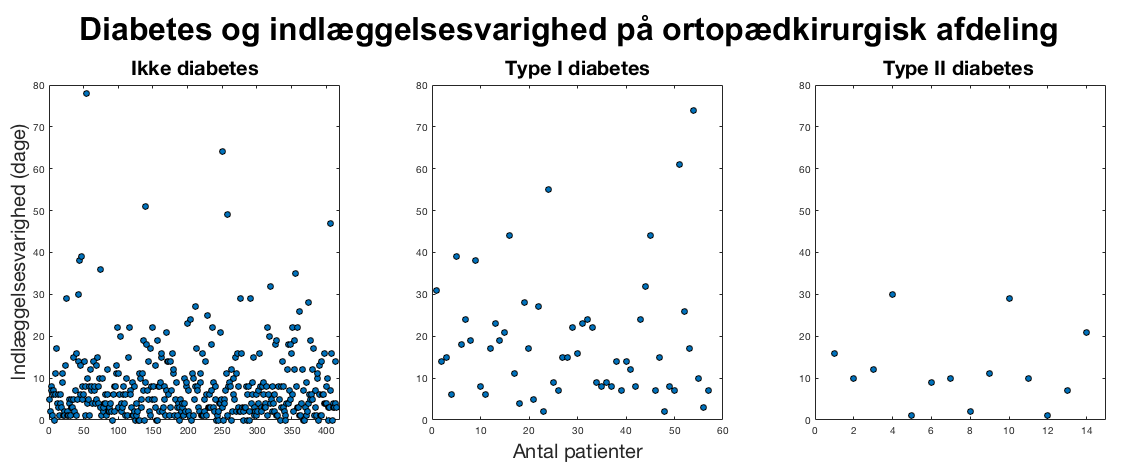
\includegraphics[scale=0.25]{figures/diabetesogindlaeg}
	%\flushleft
	\caption{\textit{Diabetes og indlæggelsesvarighed for patienter på ortopædkirurgisk afdeling. Diabetes er opdelt i ikke diabetes, type I og type II. Dette er over en periode på 3 måneder fra den 1. august til den 31. oktober år 2014. }}
	\label{diabetesogindlaeggelse}
\end{figure}

\noindent
På \figref{diabetesogindlaeggelse} ses det, at type II diabetikere har en længere indlæggelsesvarighed end type II diabetikere. Den gennemsnitlige indlæggelsesvarighed for ikke diabetikere er 7,8 dage, mens den for type I og type II diabetikere er henholdsvis 18,8 og 12,1 dage. Det tyder derfor på, at der er en sammenhæng mellem diabetes og indlæggelsesvarigheden. 

Denne sammenhæng undersøges ved en to sample t-test. Resultatet heraf fremgår af \ref{diabetesindlaegtab}

\begin{table}[H]
\centering
\begin{tabular}{|c|c|c|c|}
\hline
\textbf{Diabetes}  & \textbf{Sub-sample} & \textbf{Indlæggelsesgennemsnit} & \textbf{P-værdi} \\ \hline
Ikke diabetiker    & 415                 & 7,85                            & 0,0159*          \\ \hline
Type I diabetiker  & 57                  & 18,77                           & 5,2136           \\ \hline
Type II diabetiker & 14                  & 12,07                           & 0,1582           \\ \hline
\end{tabular}
\caption{Statistik over sammenhæng mellem indlæggelsesvarigheden og diabetes. P-værdier under et signifikantsniveau på 5\% er angivet med *.}
\label{diabetesindlaegtab}
\end{table}

\noindent
Det fremgår af \ref{diabetesindlaegtab}, at ikke diabetikere har en statistisk indflydelse på indlæggelsesvarigheden. Modsat er der ingen statistik sammenhæng mellem diabetiker og indlæggelsesvarigheden for patienterne. Patienter der er ikke diabetikere er i gennemsnit indlagt kortere tid. Der er derfor en statistisk sammenhæng mellem at være ikke diabetiker og indlæggelsesvarigheden.

\subsubsection{Kliniske faktorer}
Udover livsstilsfaktorer tyder det på at kliniske faktorer har en indflydelse. Som beskrevet i \ref{kap_OA} udføres flere operationstyper med forskellig varighed på ortopædkirurgisk afdeling, hvorfor det forventes at indlæggelsesvarigheden ligeledes er varierende. 


\begin{figure}[H]
	%\flushleft 
	\centering
	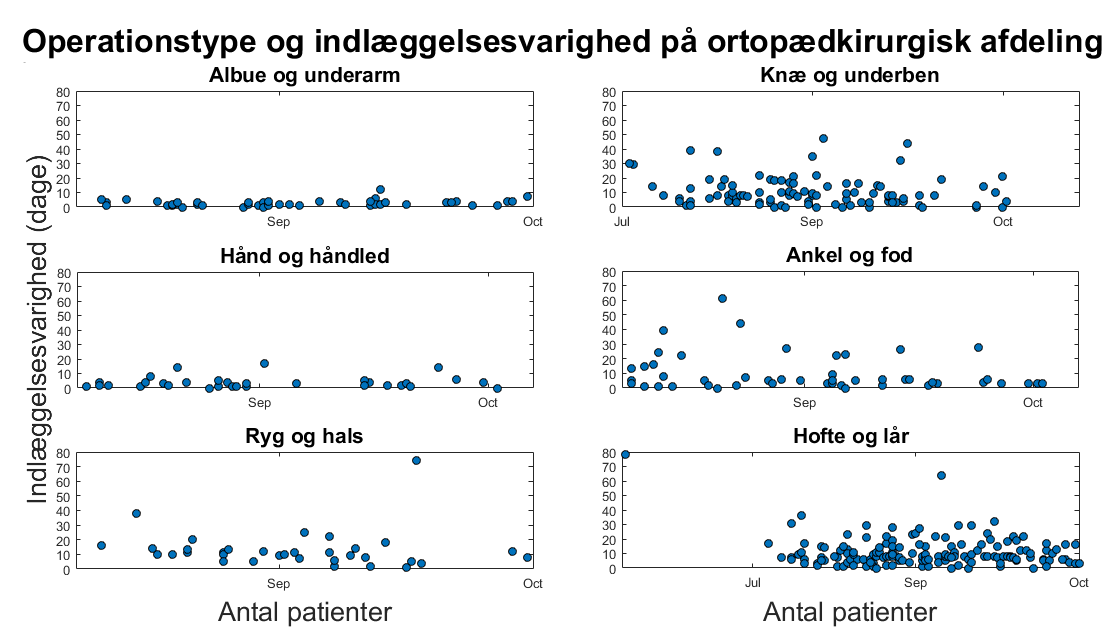
\includegraphics[scale=0.5]{figures/operaogindlaeg}
	%\flushleft
	\caption{\textit{Operationstyper og indlæggelsesvarighed for patienter på ortopædkirurgisk afdeling. Operationstyper er opdelt i albue og underarm, hånd og håndled, ryg og hals, knæ og underben, ankel og fod samt hofte og lår. Dette er over en periode på 3 måneder fra den 1. august til den 31. oktober år 2014.}}
	\label{opvsindlaegtid}
\end{figure}


\noindent
På \figref{opvsindlaegtid} fremgår det, at indlæggelsesvarigheden er varierende for typen af operationer, hvoraf den gemmesnitlige indlæggesesvarighed er fra 2,7 op til 12,5 dage. Den gennemsnitlige indlæggelsesvarighed er for ryg og hals, hofte og lår, knæ og underben samt ankel og fod, henholdsvis 12,5, 10,8, 10,2 og 10,1 dage. Modsat er den gennemsnitlige indlæggelsesvarighed for hånd og håndled samt albue og underarm 3,8 og 2,7 dage. Hertil tyder det på, at indlæggelsesvarigheden er længere for operationer foretaget på underekstremiteter sammenlignet med overekstremiteter. Derudover ses det, at de fleste operationer der foretages på ortopædkirurgisk afdeling er  hofte og lår samt knæ og underben operationer. 

For at teste for om der er signifikant sammenhæng mellem operationstypen og indlæggelsesvarighed, foretages en to sample t-test. Resultaterne af denne test fremgår af \tabref{optypeogindlaegtab}.

\begin{table}[H]
\centering
\begin{tabular}{|c|c|c|c|}
\hline
\textbf{Operationstype} & \textbf{Sub-sample} & \textbf{Indlæggelsesgennemsnit} & \textbf{P-værdi} \\ \hline
Hånd og håndled   & 34                  & 3,74                            & 5,9083           \\ \hline
Albue og underarm & 50                  & 2,72                            & 0,0011*          \\ \hline
Ankel og fod      & 49                  & 10,10                           & 0,2964           \\ \hline
Knæ og underben   & 100                 & 10,20                           & 0,2015           \\ \hline
Hofte og lår      & 157                 & 10,78                           & 0,0532*          \\ \hline
Ryg og Hals       & 37                  & 12,46                           & 0,0378*          \\ \hline
\end{tabular}
\caption{Statistik over sammenhæng mellem indlæggelsesvarigheden og operationstype. P-værdier under et signifikantsniveau på 5\% er angivet med *.}
\label{optypeogindlaegtab}
\end{table}

\noindent
Af \ref{optypeogindlaegtab} fremgår det, at  operation som albue og underarm, hofte og lår samt ryg og hals har statistisk indflydelse på indlæggelsesvarigheden. Patienter får foretaget en  albue og underarm operation er indlagt kortere tid end gennemsnittet. Hvorimod patienter er indlagt længere tid end gennemsnittet ved hofte og lår samt ryg og hals operationer. Der er derfor en statistik sammenhæng mellem disse operationer og indlæggelsesvarigheden. 


\subsubsection{Tilgængelige kirurger}
Foruden livsstilsfaktorer og operationstype kan tilgængeligheden af kirurger have indflydelse på indlæggelsesvarigheden for patienterne. Det kan i nogle tilfælde være nødvendigt at udsætte elektive patienters operationer, hvis et akut tilfælde opstår, hvorved kirurgen skal være til stede. Derved kan patienter indlæggelsesvarighed forlænges. Ved udsættelse af elektive patienter vil denne ofte få en ny tid hurtigst muligt. Den nye tid vil typisk være først på dagen, således risikoen for endnu en udsættelse mindskes.\ref{bilagA}